\section{Methodology}
\label{sec:methodology}


\subsection{Data Preprocessing}
In some situations, it becomes difficult to measure the physical properties of a particle such as momentum and energy accurately. In our original dataset, as many as 177000 out of 250000 instances had missing attributes. We considered three approaches to deal with missing values. First, we tried ignoring instances with missing attributes. But this resulted in very few useful instances. Second, we tried to replace the missing values with the mean/median. However, this biases the experiments. Finally, we decided to adopt a method known as multiple imputations~\cite{MultipleImputation} which replaces the missing values with a random number that follows the distribution for that attribute. We use the \texttt{Amelia}~\cite{Amelia} package to perform this task.



\subsection{Feature Engineering and Selection}

\begin{figure*}[t]
\centering
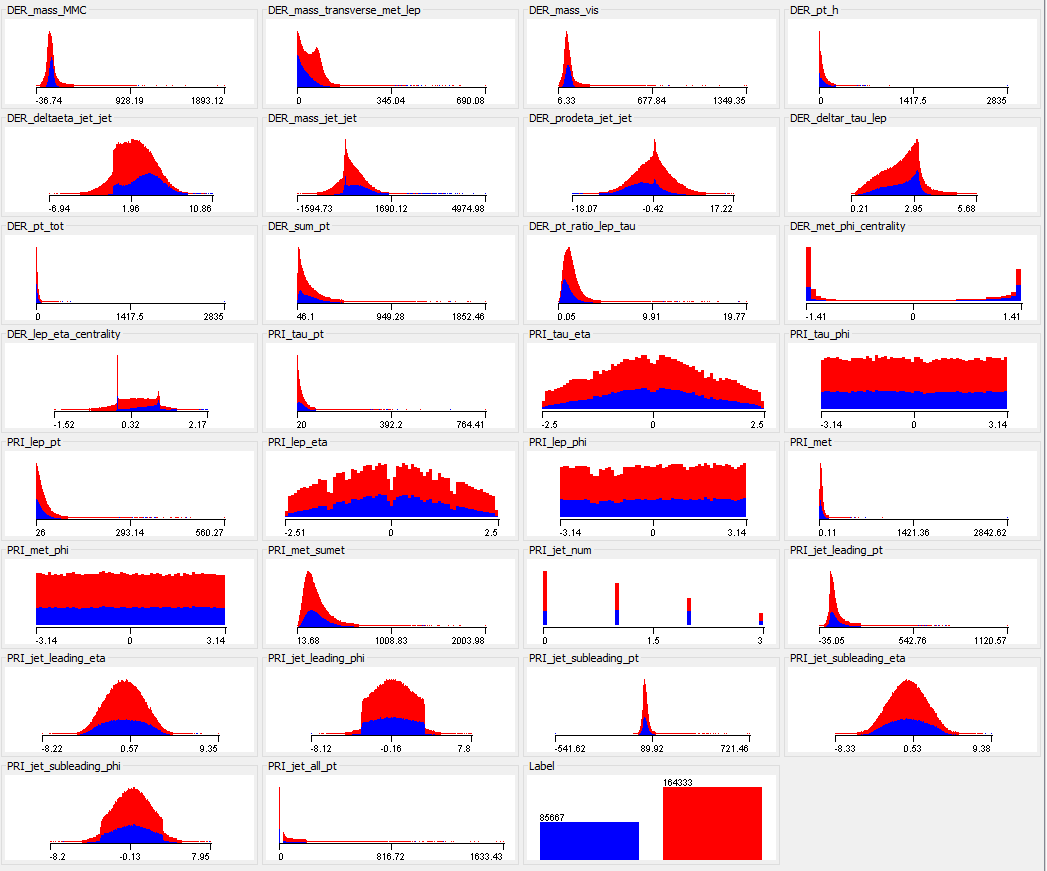
\includegraphics[width=1.8\columnwidth]{Distribution}
\caption{Distribution of different attributes for signal. Blue represents signal and red represents background.}
\label{fig:distribution}
\end{figure*}

The raw dataset includes 17 features. From these 17 basic features, 13 additional features were derived. These 13 derived features describe some property of the particle and requires knowledge of physics. The features are provided by physics. Their description is given in the appendix. From these 30 features, a subset is selected based on the following factors. First, we decide the ability of the feature/attribute to distinguish between signal an background. The distribution of different attributes is shown in Fig.~\ref{fig:distribution} for signal and background separately. Second, we try to avoid using features correlating with each other while building the classifier. Fig.~\ref{fig:correlation-matrix} shows the correlation matrix of the features. The final set of features selected differs for each classifier. The details are given in their respective subsections.

\begin{figure}[h]
\centering
\includegraphics[width=1.0\columnwidth]{corr}
\caption{Correlation matrix. Dark blue indicates features that shows strong positive correlation. Dark red indicates features that show strong negative correlation.}
\label{fig:correlation-matrix}
\end{figure}



\subsection{Data Analytics Techniques}

In this section, we describe the various classification schemes we explored. For each technique, we also describe the parameter settings explored in brief.


\subsubsection{Bayesian Classifiers}

\paragraph{Naive Bayes}

This classifier is based on the Naive Bayes technique developed by John et al.~\cite{NaiveBayes}. The modeling and prediction overhead were negligible as this method is known to be highly scalable. This method could classify background noise better when compared to signal. During data preprocessing step, we included only those features whose Pearson correlation coefficient was below a particular threshold. Our experiments suggested that out by increasing the threshold value, which in turn increases of number of correlated features, resulted in decrease in the performance of this method.The best performance is achieved when the dataset included 12 features whose pairwise correlation coefficient is less than 0.6.	

\subsubsection{Functions-based Classifiers}

\paragraph{Logistic Regression}

This classifier is based on the Ridge estimation technique developed by Cessie et al.~\cite{Logistic Regression}. Being a linear method, the modeling and prediction overhead were small. In this technique, we used L1 regularized logistic regression. We explored the performance of this method
by varying the number of features in the dataset. The results on our dataset suggest that performance seems to be more or less the same with varying number of features.

\paragraph{Linear Discriminant Analysis}

This linear classifier fits a gaussian distribution of equal variance to each of the classes. We took the class priors to be equal when evaluating this method. The results on our dataset indicate that performance of this technique remains more or less the same when number of features are varied.

\paragraph{Quadratic Discriminant Analysis}

This linear method is similar to Linear Discriminant Analysis, expect that this technique uses quadratic decision boundaries. In evaluating this method, we used equal class priors. The optimal performance shown in the table is obtained when the dataset included features whose pairwise correlational coefficient is less than 0.95.

\subsubsection{Tree-based Classifiers}

\paragraph{Decision Tree Classifier}

In evaluating the performance of decision tree classifier, we used "gini" and "entropy" criterion.These two criterion on our dataset produced similar results. We varied the minimum number of samples required to split an internal node, and the best performance was achieved when this value was 300.  The optimal results for this classifier are shown in the table.

\subsubsection{Instance-based Classifiers}

\paragraph{k-Nearest Neighbor}

For the instance-based classifier we explore the k-nearest neighbor (kNN) technique~\cite{kNN}. This is a lazy classification technique in which the \emph{k} nearest neighbors are looked at to decide the class of a new instance. This technique has practically no training overhead. The classification overhead is very high though, particularly if the distance for all previously seen instances are computed exhaustively. Since this technique is known to perform bad with noisy attributes and irrelevant attributes, we explore removing such attributes from our dataset. We also tried to construct the classifier using top few principal components in order to keep only relevant features. In addition, we also experiment with the number of neighbors considered.


\subsubsection{Neural Networks}

For Higgs Boson project, we used both deep and shallow neural networks. We analyzed our data using multiple networks each of which are discussed below. 


\paragraph{feedforwardnet} Feed Forward networks consist of a series of layers. The first layer has a connection from the network input. Each subsequent layer has a connection from the previous layer. The final layer is the output layer which produces the network output. 
The hidden layer is of size 60. The transfer function used in this layer is 'tansig' (tan-Sigmoid Transfer Function). Tansig is a neural network transfer function which calculates a layer's output from its net input. The output layer produces only 1 output ( 0 or 1). The transfer function used in this layer is 'purelin'. It is a linear transfer function which calculates the final output.


\paragraph{patternet} It is a Pattern Recognition Network which is trained to classify inputs from target classes. The target data should consist of a vector of 0 or 1. It contains one hidden layer of size 40. The output layer is of size 1.


\paragraph{cascadeforwardnet}  Cascade Forward Network is very similar to feed forward networks but includes a connection from the network input and from every previous layer to following layers. The output layer has two inputs : one from the previous hidden layer and the other from the input. The hidden layer is of size 80. The rest of the network is same as that of FeedForwardNetwork.  


\paragraph{Custom Neural Network}  We designed a deep neural network with 4 layers: three hidden layers, one output layer. All the hidden layers are connected to the network input.  There is no direct connection between any of the three hidden layers. The output layer takes 4 inputs, three of the inputs are outputs of each hidden layer. The output layer is also recursive layer. So it's own output is fed back as its fourth input. The network model is trained using 'trainrp' network training function which updates weight and bias according to resilient back propagation algorithm (Rprop).
The 1st hidden layer contains 20 neurons. The transfer function used in this layer is 'tansig' (tan-Sigmoid Transfer Function). The second hidden layer has 10 neurons. The transfer function used here is 'logsig'. It is log-sigmoid transfer function. The third hidden layer has 20 neurons. The transfer function used here is again 'tansig'.  The output layer produces only 1 output ( 0 or 1). The transfer function used in this layer is 'purelin'.


The number of layers in a network, number of neurons in each layer, transfer function to be used to calculate output of each layer, etc are based on heuristics. We have used biases in the network as networks with biases are more powerful. Each layer's weights and biases are initialized with the Nguyen-Widrow layer initialization method~\cite{NN-Speed}.




\subsubsection{Meta Classifiers and Ensemble Methods}

\paragraph{Classification via Clustering and Regression}

We simply cluster the raw dataset and mark certain clusters as signal and others as noise. Prediction based on the distance of the new data point to the centroid of the two cluster groups.  For the regression technique, we form an equation from the basic parameters and based on the value from the equation, we predict if the event is a signal or a background.

\paragraph{Bagging}

Bagging technique developed by Brieman involves creating several models using different subsets of the training dataset~\cite{Bagging}. Each model does its own classification and they all vote with equal weight to decide on the class. We explored the number of iterations it takes to form the solution. We also experimented with two types of tree based classifiers - REP Tree and Decision Stump Classifier.


\paragraph{Boosting}

Boosting is similar to bagging in that we create several models and they all vote to make the final decision. However, there is a difference in how the dataset is constructed for each model. All those instances that failed in model 1 are propagated to subsequent models. The models that come later all try to improve the regions where the older models failed. Here we explore ADA Boosting developed by Freund and Schapire~\cite{ADABoosting} and MultiBoosting technique developed by Webb~\cite{MultiBoosting}. We use these techniques in conjuction with REP Tree and Decision Stump Tree classifiers.

\paragraph{Rotation Forest}

Rotation Forest is an ensemble method developed by Rodriguez et al.~\cite{RotationForest} where several classifiers are combined to produce a highly accurate classifier. Here, again several decision trees combine to decide the final class. However, the difference here is that each tree does this classification based on a \emph{different} subset of the \emph{principal components}. We use this technique in conjunction with J48 decision tree and REP Tree.


